\documentclass[11pt]{article}
%%%%%%%%%%%%%%%%%%%%%%%%%%%%%%%%%%%%%%%%%%%%%%%%%%%%%%%%%%%%%%%%%%%%%%%%%%%%
% Nick Waters's super awsome template for biorXiv submissions

% In memory of Henry, Hermine, and Angus.
% May there be many tasty snails in pufferfish heaven
%%%%%%%%%%%%%%%%%%%%%%%%%%%%%%%%%%%%%%%%%%%%%%%%%%%%%%%%%%%%%%%%%%%%%%%%%%%%
\usepackage{geometry}
\geometry{marginparwidth=1cm,a4paper,verbose,tmargin=1.5cm,bmargin=1.5cm,lmargin=1.5cm,rmargin=1.5cm,headheight=0cm,headsep=0cm,footskip=0cm}
\usepackage{cite}
\setlength\parindent{0pt} % set indent to zero
\setlength{\parskip}{1.2em} % give a bit of space between paragraphs

\bibliographystyle{plain} % citation and bib style
\usepackage{grffile} %for underscores in file names
\usepackage[ruled]{algorithm2e} % for typesetting the riboSeed algorithm
\setlength{\algotitleheightrule}{0pt}
\usepackage{lineno, color} % controls line numbering
% \linenumbers % just in body, not in bibliography or abstract
\modulolinenumbers[5]  % number every 5th line
% format our line numbers, cause no one likes boring numbers
\renewcommand\linenumberfont{\normalfont\tiny\color{blue}}

\usepackage{booktabs}  % less yucky tables
% nice little thing for table spacing (thanks Markus Püschel)
\newcommand{\ra}[1]{\renewcommand{\arraystretch}{#1}}

\usepackage{multirow}
% my lined-off abstract
\newenvironment{myabstract}{%
\begin{quote} \baselineskip15pt \rule{.89\textwidth}{1.5pt} \vskip .22cm}
{ \vskip .04cm \rule{.89\textwidth}{1.5pt} \end{quote}}
% supplementary (essentialy just resets numbering)
\newcommand{\beginsupplement}{%
        \setcounter{table}{0}
        \renewcommand{\thetable}{S\arabic{table}}%
        \setcounter{figure}{0}
        \renewcommand{\thefigure}{S\arabic{figure}}%
     }


%   This forces numbering of subsections but not sections
\usepackage{titlesec}% http://ctan.org/pkg/titlesec
\titleformat{\section}%
  [hang]% <shape>
  {\normalfont\bfseries\Large}% <format>
  {}% <label>
  {0pt}% <sep>
  {}% <before code>
\renewcommand{\thesection}{}% Remove section references...
\renewcommand{\thesubsection}{\arabic{subsection}}%... from subsections


\usepackage[%
    % font={small,sf},
    font={small},
    labelfont=bf,
    format=hang,
    format=plain,
    margin=0pt,
    width=0.9\textwidth,]{caption}
\usepackage[list=true]{subcaption}

\title{\fontseries{m}\selectfont riboSeed: leveraging prokaryotic genomic architecture to assemble across ribosomal regions}



\author
{\small Nicholas R Waters,$^{1,2\ast}$ Florence Abram,$^{1}$  Ashleigh Holmes,$^{2}$ Fiona Brennan,$^{1,3}$ and Leighton Pritchard$^{2}$\\
\\
\normalsize{\textit {$^{1}$National University of Ireland, Galway}}\\
\normalsize{\textit {$^{2}$The James Hutton Institute, Dundee, Scotland}}\\
\normalsize{\textit {$^{3}$Teagasc, Johnstown Castle, Wexford}}\\
\\
\footnotesize{$^\ast$To whom hate mail should be addressed; E-mail: n.waters4@nuigalway.ie.}
}
\date{}

\usepackage{graphicx}
\graphicspath{ {riboFigs/} }

\begin{document}
\baselineskip20pt  % set line spacing; double spacing is 2xfontsize, in this case 11
\maketitle


\begin{myabstract}
The vast majority of bacterial genome sequencing has been performed using Illumina short reads. Because of the inherent difficulty of resolving repeated regions with short reads alone, only 10\% of sequencing projects have resulted in a closed genome. The most common repeated regions are those coding for ribosomal operons (rDNAs), which can occur in a bacterial genome between 1 and 15 times, and are commonly used as sequence markers to classify and identify bacteria. Here, we show that the genomic context in which rDNAs occur is conserved across taxa and that, by utilizing the conserved nature of rDNAs across taxa and the uniqueness of their flanking regions, it is possible to improve assembly of these regions relative to de novo sequencing. We describe a method which constructs targeted pseudocontigs generated by iteratively assembling reads that map to a reference genome’s rDNAs. These pseudocontigs are then used to more accurately assemble the newly-sequenced chromosome. We show that this method, implemented as riboSeed, correctly bridges across adjacent contigs in bacterial genome assembly and, when used in conjunction with other genome polishing tools, can result in closure of a genome.
\end{myabstract}

Keywords: genome assembly, ribosome, benchmarking, scaffolding, de fere novo

\begin{linenumbers}


\section*{Background}
\begin{table}[]
\centering
\caption{NCBI Genome Assemblies of Bacteria}
\label{table:completions}
\begin{tabular}{llllll}
  Date              & Total & Complete genome & Chromosome & Scaffold & Contig \\
  \hline
January 4th, 2017 & 85799 & 6255            & 1143       & 39972    & 38429  \\
May 17th, 2017    & 96849 & 7212            & 1254       & 42839    & 43899

\end{tabular}
\end{table}

Sequencing bacterial genomes has become much more cost effective and convenient, but the number of complete, closed bacterial genomes remains a small fraction of the total number sequenced (Table \ref{table:completions}). The length of short reads is increasing, but even with the advent of new long-read technologies, bacterial assembly remains a major bottleneck\cite{Nagarajan2010,Brouwer2016}. Although draft genomes are often of very high quality and suited for many types of analysis, researchers are forced to choose between working with these draft genomes (and the inherent potential loss of data), or spending time and resources polishing the genome with some combination of in silico tools, PCR, optical mapping, resequencing, or hybrid sequencing\cite{Nagarajan2010,Utturkar2014}. Many in silico genome finishing tools are available, and we summarise several of these in Table \ref{table:tools}.




\begin{table}[]
\centering
\caption{Alternative in silico genome polishing tools}
\label{table:tools}
\resizebox{\textwidth}{!}{
\begin{tabular}{llp{9cm}}
  Tool & Reference & Method Summary \\
  \hline
  GapFiller & Boetzer2012\cite{Boetzer2012} & utilizes paired end and other short read information to close contig junctions \\
  % SOAPdenovo2’s
  GapCloser/IMAGE & Luo2012, Tsai2010\cite{Luo2012, Tsai2010} & iteratively uses reads that are mapped to contigs, to close contig junctions \\
  CloG & Yang2011\cite{Yang2011} & use trimmed de novo contigs in hybrid assembly followed by a stitching algorithm \\
  FGap & Piro2014,Guizelini2016\cite{Piro2014,Guizelini2016} & uses BLAST to find potential gap closures from alternate assemblies, libraries or references. \\
  GFinisher & Guizelini2016\cite{Guizelini2016} & uses GC-skew to refine assemblies \\
  GapFiller & Nadalin2012\cite{Nadalin2012} & local assembler using a hash-based method to produce “long-reads” from paired end sequencing data, which can then be used in a de novo assembly. \\
  CONTIGuator & Galardini2011\cite{Galardini2011} & uses contigs from a de novo assembly along with one or more reference sequences to generate a contig map and PCR primer sets to validate in the lab. \\
  Konnector & Vandervalk2015 \cite{Vandervalk2015} & uses paired end reads to make long reads to be used in a Bloom filter representation of a de Bruijn graph \\
  MapRepeat & Mariano2015\cite{Mariano2015} & uses a directed scaffolding method to fill in rDNA gaps, but limited to Ion Torrent reads, and affected by inversions between rDNAoperons \cite{Mariano2016} \\
  GRabB & Brankovics2016\cite{Brankovics2016} & selective assembly tandem rDNA clusters and mitochondria
\end{tabular}
}
\end{table}



The Illumina entries in NCBI’s Sequence Read Archive (SRA) \cite{Kodama2012} outnumber all other technologies combined by about an order of magnitude (sup table 3). Draft assemblies from these datasets have systematic problems common to short read datasets, namely gaps in the sequences due to the difficulty of resolving assemblies of repeated regions\cite{Whiteford 2005, Treangen 2013}. By improving the ability to resolve assemblies through repeated regions  it may be possible to improve on current assemblies, and therefore obtain additional sequence information from existing short read datasets in the SRA.,.



The most common repeated regions are those coding for ribosomal RNAs. Sequencing of the 16S ribosomal region is widely used to identify bacteria and explore microbial community dynamics\cite{Weisburg1991,Clarridge2004,Woese1990,Case2007}, as the region is conserved within taxa, yet retains enough variability to act as a bacterial “fingerprint” to separate clades informatively. However, the 16S, 23S, and 5S ribosomal subunit coding regions (rDNA) are often present multiple times in a single prokaryoticgenome, and commonly exhibit polymorphism \cite{Coenye2003,Moreno2002,Lukjancenko2010,Větrovský2013}. These long, inexactly repeated regions\cite{Agrawal2016,Alkan2011} are problematic for short-read genome assembly. Other large repeated regions also exist, but none as pervasive as rDNAs, as ribosomes are essential for cell function. As rDNAs are frequently used as a sequence marker for taxonomic classification, resolving their copy number and sequence diversity from short read collections where the assembled genome has collapsed several repeats into a single region could increase the accuracy of community analysis. We present here an in silico method, riboSeed, that capitalizes on the genomic conservation of rDNA regions within a taxon to improve resolution of these normally difficult regions and provide a means to benefit from unexploited information in the SRA/ENA short read archives.


riboSeed is most similar in concept to GRabB, the method of Brankovics et. al \cite{Brankovics2016} for assembling mitochondrial and rDNA regions in eukaryotes, as both use targeted assembly. However, GRabB does not make inferences about the number of rDNA clusters present in the genome, or take advantage of their genomic context. In riboSeed, genomic context is resolved by exploiting both rDNA regions and their flanking regions, harnessing unique characteristics of the broader rDNA region within a single genome to improve assembly.


The riboSeed algorithm proceeds from two observations: (1) that although repeated bacterial rDNA coding sequences within a single genome are nearly identical, their flanking regions (ie, the neighboring locations within the genome), are distinct, and (2) that the genomic contexts of rDNAs  are conserved within a taxonomic grouping. riboSeed uses only reads that map to rDNA regions from a reference genome, and is not affected by chromosomal rearrangements that occur outside the flanking regions immediately adjacent to each rRNA.


Briefly, riboSeed uses rDNA regions from the closest completely sequenced reference genome to generate rDNA cluster-specific “pseudocontigs” that are seeded into the raw short reads to generate a final assembly. We refer to this process as de fere novo (meaning 'starting from almost nothing') assembly.


\begin{figure}[h]
    \centering
    \includegraphics[width=0.75\textwidth]{riboSeed_v11}
    \caption{Reads are mapped to a reference genome and those reads that align to rDNA and flanking regions are extracted. A subassembly for each group of reads that maps to an rDNA region is constructed to produce a “pseudocontig” for each region. These pseudocontigs are then concatenated together separated by 5kb of N’s as a buffer. Reads are then iteratively mapped to the concatenated pseudocontigs, extracted, and again subassembled to each region. After the final iteration, the pseudocontigs are included with raw reads in a standard de novo assembly. The complete process is referred to as de fere novo assembly. The subassemblies attempt to bridge proper rDNA regions by ensuring that flanking regions (represented here by colors) remain correctly paired.
}
    \label{fig:overview}
\end{figure}




\section*{Implementation}
We present riboSeed: a software suite that allows users to easily perform de fere novo assembly, given a reference genome sequence and single or paired end Illumina sequence reads . The code is primarily written in Python3, with several accessory shell and R scripts.


riboSeed relies on a closed reference genome assembly that is sufficiently closely-related to the isolate being assembled, in which rDNA regions are assembled and known to be in the correct context(see FIGURE 3).

riboSeed proceeds in three stages: preprocessing, de fere novo assembly, and assessment/visualization.
\subsection*{1. Preprocessing}
\subsubsection*{riboScan.py}


riboScan.py uses Barrnap[Seemann2014] to annotate rDNAs in the reference genome, and EMBOSS’s seqret[Rice2000] to create GenBank, FASTA, and GFF formatted versions of the reference genome. This preprocessing step unifies the annotation vocabulary for downstream processes.

\subsubsection*{riboSelect.py}
riboSelect.py attempts to infer rDNA operon structure from the genomic location of constituent 16S, 23S and 5S sequences. The number of 16S sequences is identified from the riboScan.py annotation, and Jenks natural breaks algorithm (using the 16S count to set the number of breaks) then employed to group rRNA annotations into likely operons on the basis of  their genomic coordinates. The output identifies individual rDNA clusters and describes their component elements in a plaintext file. This output can be easily adjusted by hand before assembly if the clustering does not appear to accurately reflect the arrangement of the operons (for example, based on visualization of the annotations in a genome browser).

\subsection*{2. De Fere Novo Assembly}
\subsubsection*{riboSeed.py}
riboSeed.py implements the algorithm described in FIGURE 2. Short reads for the sequenced isolate are mapped to the reference genome using BWA[Li 2009]. Reads that map to each annotated rDNA cluster and its flanking regions (default size 1kbp) are extracted into subsets (one per cluster). Each subset of extracted reads (one per cluster) is assembled into a representative pseudocontig with SPAdes[Bankevich2012], using the reference rDNA regions as a trusted contig. The resulting pseudocontigs are evaluated for inclusion in future mapping/subassembly iterations based on their length (as discussed below), and concatenated into a pseudogenome, in which pseudocontigs are separated by 5kb of Ns as a buffer.


This process is repeated in each subsequent iteration, using the pseudogenome as the reference, and the pseudocontig as a trusted contig.


After a specified number of iterations (3 by default), SPAdes is used to assemble all short reads in a hybrid assembly that includes the pseudocontigs from the final iteration as trusted contigs (or as ‘untrusted contigs’ if the mapping quality of reads to that pseudocontig falls below a threshold). As a control, the short reads are also de novo assembled without the pseudocontigs.


Although riboSeed uses SPAdes to perform both the subassemblies and the final de fere novo assembly, the pseudocontigs could be submitted to any hybrid assembler that accepts short read libraries and contigs. After assembly, the de fere novo and de novo assemblies are assessed with QUAST[Gurevich2013].

%%%%%%%%%%%%%%%%%%%%%%%%%%%%%%%%%%%%%%%%%%%%%%%%
\SetKwProg{Scan}{riboScan}{ }{end}
\SetKwProg{Select}{riboSelect}{ }{end}
\SetKwProg{Seed}{riboSeed}{ }{end}
\begin{figure}[h]
  \centering
  \begin{minipage}{.6\linewidth}
    \begin{algorithm}[H]
      % \KwData{reference, reads}
      %  % initialization\;
      % \Scan{(reference fastas)}{
      % \For{chromosome in reference}{
      % run Barrnap to find rRNAs\;
      % add locus tags to gff\;
      % convert to genbank\;
      % }
      %   combine genbanks\;
      %   return scannedScaffolds\;
      % }
      %   \hrule
      % % \end{algorithm}
      % % \pagebreak
      % % \begin{algorithm}[H]
      %   \Select{(scannedScaffolds)}{
      %   parse coordinated of rRNAs\;
      %   cluster into operons\;
      %   return grouped\_loci\;
      % }
      %   \hrule
      % \end{algorithm}
      % \pagebreak
      % \begin{algorithm}[H]
      %   \Seed{(scannedScaffolds, grouped\_loci, reads, iters)}{
      %   reference = scannedScaffolds\;
      %   clusters = parse grouped\_loci\;
      %   \For{i in iters}{
      %   map reads to reference\;
      %   \For{cluster in clusters}{
      %   filter and extract reads within clusters and flanking\;
      %   subassemble with SPAdes\;
      %   return pseudocontig\;
      % }
      %   assess subassembly\;
      %   \If {success}{
      %   make fauxgenome from pseudocontigs \;
      %   reference = fauxgenome
      %   continue
      % }
      %   \If{last iteration}{
      %   run SPAdes with pseudocontigs\;
      % }
      % }
      % }
      \Seed{(reference, riboSelect\_clusters, reads, iters)}{
        ref = reference\;
        clusters = parse riboSelect\_clusters\;
        \For{i in iters}{
          map reads to ref\;
          \For{cluster in clusters}{
            filter and extract reads within clusters and flanking\;
            subassemble with SPAdes\;
            return pseudocontig\;
          }
          assess subassembly\;
          \If {success}{
            make pseudogenome from pseudocontigs \;
            ref = pseudogenome \;
          }
        }
        run SPAdes with reads and pseudocontigs\;
      }
    \end{algorithm}
  \end{minipage}
  \label{fig:algo}
  \caption{Pseudocode of riboSeed algorithm}
\end{figure}
%%%%%%%%%%%%%%%%%%%%%%%%%%%%%%%%%%%%%%%%%%%%%%%%%%%% 5


\subsection*{3. Assessment and Visualization}
\subsubsection*{riboScore.py}
riboScore.py extracts the regions flanking the rDNAs in the reference and in the assemblies generated by riboSeed. The rDNA flanking regions from an assembly are aligned to rDNA flanking regions reference regions using BLAST, and depending on the scoring of the alignments, calls a junction a successful join, a misassembly, or ambiguous based on the criteria outlined below.
\subsubsection*{riboSnag.py}
riboSnag.py is provided as a helper tool to produce useful diagnostics and visualisation concerning rDNA sequence in the reference genome. Using the clustering generated by riboSelect.py, sequences for the clusters can be extracted from the genome, aligned, and Shannon entropy [Schmitt1997] plotted with consensus depth for each position in the alignment.
\subsubsection*{riboSwap.py}
In all cases, we recommend assessing the performance of the riboSeed pipeline visually using Mauve[Darling2004,Darling2011], Gingr[Treangen2014], or a similar genome assembly visualizer to compare reference, de novo, and de fere novo assemblies in addition to riboScore, If contigs appear to be incorrectly joined, the offending de fere novo contig can be replaced with syntenic contigs from the de novo assembly using the riboSwap.py.


\subsubsection*{riboStack.py}
riboStack.py uses bedtools[Quinlan2010] and samtools[Li2009] to compare the depths of coverage in the rDNA regions to randomly sampled regions elsewhere in the reference genome. riboStack.py takes output from riboScan.py, and a BAM file of reads that map to the reference. If the number of riboScan.py-annotated rDNAs matches the number of rDNAs in the sequenced isolate, the coverage depths within the rDNAs will be similar to other locations in the genome. If the coverage of rDNA regions sufficiently exceeds the average coverage elsewhere in the genome, this may indicate that the reference strain has fewer rDNAs than the sequenced isolate. In this case, using an alternative reference genome may produce improved results.
Results



\section*{Results}
\subsection{Characteristics of rDNA flanking regions}
The ability to use rDNA flanking sequences to uniquely identify and place rDNA regions in their genomic context requires the flanking sequences to be distinct within the genome for each region. This is expected to be the case for most, if not all, prokaryotic genomes. To demonstrate this, rDNA and 1-kb flanking regions were extracted from E. coli Sakai[Hayashi2001] (BA000007.2), in which the rDNA operons have been well characterized[Ohnishi2000]. These regions were aligned with MAFFT[Katoh2002], and their consensus depth and Shannon entropy calculated for each position in the alignment[Schmitt1997].


In MG1655, the first rDNA operon is located 363 bases downstream of gmhB (locus tag b0200). Homologous rDNA regions were extracted from 25 randomly selected complete E. coli chromosomes(S TABLEX)  We identified the 20kb region surrounding gmhB in each of these genomes, then annotated and extracted the corresponding rDNA operon and flanking sequences. These sequences were aligned with MAFFT, and the Shannon entropies and consensus coverage plotted.


\begin{figure}[h]
    \centering
    \begin{subfigure}[b]{.9\textwidth}
      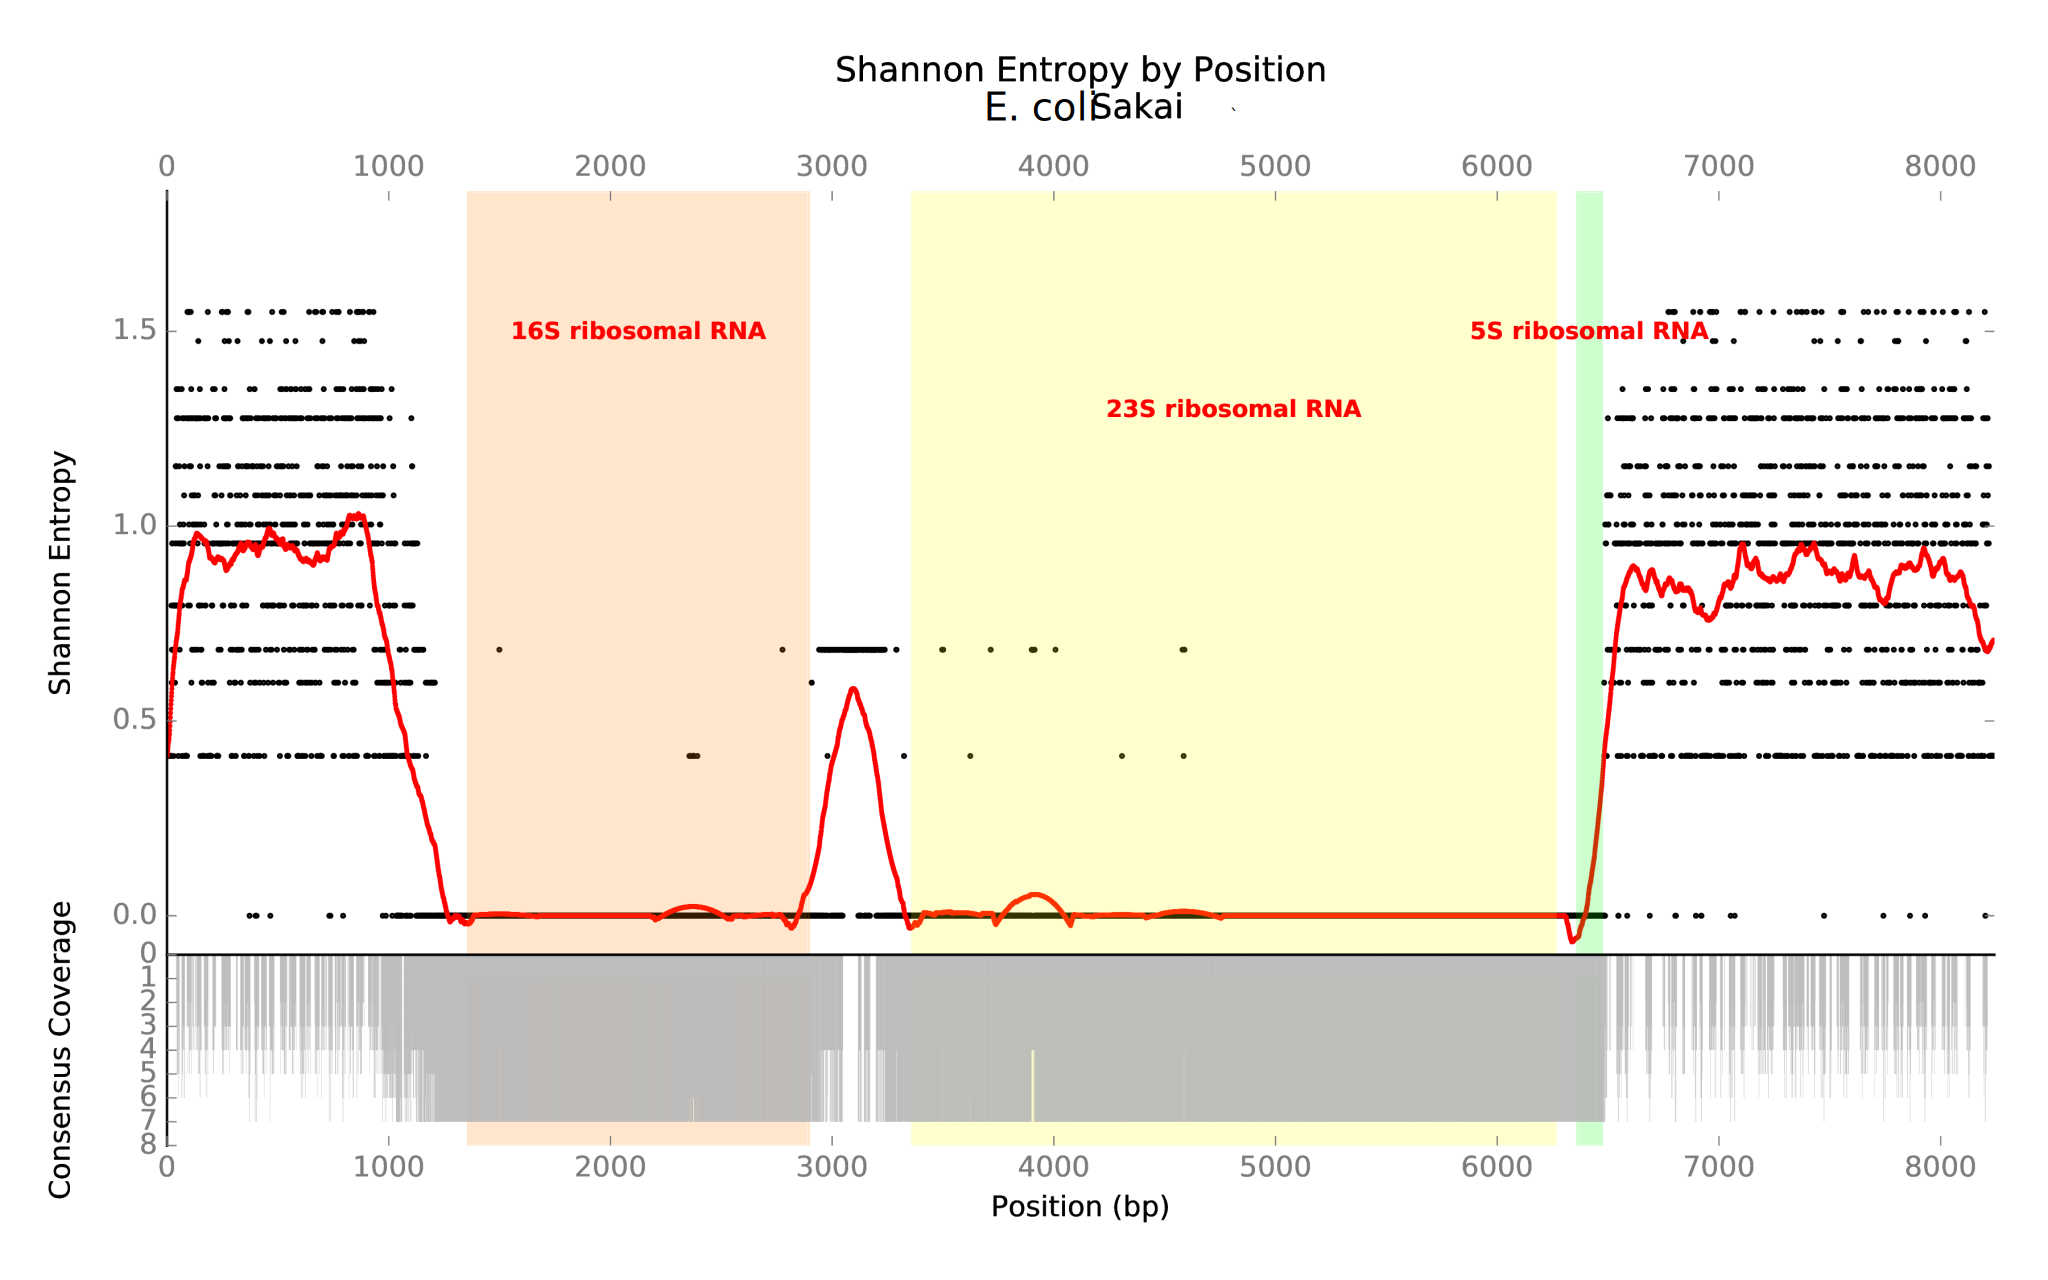
\includegraphics[width=0.7\textwidth]{entropy_plot}
      \caption{}
      \label{fig:Ng1}
    \end{subfigure}
    \begin{subfigure}[b]{.9\textwidth}
      \includegraphics[width=0.75\textwidth]{entropy_plot_gmbH}
      \caption{}
      \label{fig:Ng2}
    \end{subfigure}

    \caption{Consensus coverage depth (grey bars) and Shannon entropy (black points, smoothed entropy as red line) for aligned rDNA regions. For the seven E. coli Sakai rDNA regions (A), entropy sharply increases moving away from the coding regions of the rDNA operon. In this case flanking regions would be expected to assemble uniquely. By contrast, the rDNA regions occurring closest to homologous gmbH genes from 25 E. coli genomes (B) show greater conservation in their flanking regions. This indicates that flanking regions are more conserved for homologous rDNA operons than for paralogous operons, and implies that related genomes are useful reference templates for assembling across these regions. (Similar plots for each of the GAGE-B genomes used later for benchmarking can be found in supplemental FIGUREs 1a-h).}
    \label{fig:entropy}
\end{figure}

FIGURE 3A shows that within a single genome the regions flanking rDNA operons are variable between operons. This enables unique placement of reads at the edges of rDNA coding sequences in their genomic context (i.e. there is not likely to be confusion between the placements of rDNA operon edges within a single genome).


FIGURE 3B (and supplementary XXX) shows that homologous rDNA regions, plus their flanking regions, are well-conserved across several related genomes. Assuming that individual rDNA operons are monophyletic within a taxonomic group, short reads that can be uniquely placed on a related genome's rDNA as a reference template are also likely able to be uniquely-placed in the appropriate homologous rDNA operon of the genome to be assembled.


Taken together, these two properties allow for unique placement of reads from homologous rDNA regions in the appropriate genomic context. These 'anchor points' then reduce the number of branching possibilities in de Bruijn graph assembly for each individual rDNA operon, and thereby permit complete assembly through the full rDNA region.


\subsection*{Validating Assembly across rDNA regions}

Settings used for analyses in this manuscript are the defaults as of riboSeed version 0.4.09 (except where otherwise noted).


To evaluate the performance of de fere novo assembly compared to de novo assembly methods, we used Mauve to visualize syntenic regions and contig breaks of the assemblies in relation to the reference genome that was used to generate pseudocontigs. We categorized each rDNA cluster in an assembly as either a success, failure, or misassembly.


An rDNA cluster was classed as a success if two criteria were met: (i) the assembly merged two contigs across a rDNA region such that, based on the reference, the flanking regions of the de fere novo assembly were syntenous with those of the reference; and (ii) the assembled contig extends at least 90% of the flanking length. An assembled cluster is defined as a failure if the ends of one or more contigs aligned within the rDNA or flanking regions (signalling that extension through the rDNA region was not possible). Finally, if two contigs assembled across a rDNA region in a manner that conflicted with the orientation indicated in the reference genome, the rDNA region was deemed to be misassembled.


In all cases, SPAdes was used with the same parameters for both de fere novo assembly and de novo assembly, apart from the addition of pseudocontigs in the de fere novo assembly.

\subsection*{Performance on Simulated Reads}
\subsubsection*{Simulated Reads with Artificial Genome}
To create a small dataset for testing, we extracted 7 distinct rDNA regions from the E. coli sp. Sakai genome BA000007.2, including 5kb upstream and downstream flanking sequence, using the tools riboScan.py, riboSelect.py and riboSnag.py. Those regions were combined to produce a ~100kb artificial test chromosome. pIRS[Hu2012] was used to generate simulated reads (100bp, 300bp inserts, stdev 10, 30-fold coverage, built-in error profile) from this test chromosome. These reads were assembled using riboSeed, with the E. coli MG1655 genome (NC\_000913.3) as a reference.  Because of the random nature of read simulation, this was repeated 8 times.


The de fere novo assembly bridged an average of 4 of the 7 rDNA regions in the artificial genome, while the de novo assembly method failed to bridge any. To demonstrate that the choice of reference sequence determines the ability to assemble correctly through rDNA contigs, we ran riboSeed with the same E. coli reads using Klebsiella pneumoniae reference pseudocontigs derived from the HS11286 (CP003200.1) genome[Liu2012] The de fere novo assembly with pseudocontigs from K. pneumoniae bridged between 0 and 3 rDNAs, but also misassembled  several rDNA gaps (FIGURE 4, SFIGURE X).

\begin{figure}[H]
    \centering
    \includegraphics[width=0.75\textwidth]{PrettyMauve}
    \caption{Mauve output describing the results of riboSeed assemblies of simulated reads generated by ART from the concatenated E. coli Sakai artificial genome. From top to bottom: artificial reference chromosome; rDNA clusters (red bars); de fere novo assembly (E. coli reference), de novo assembly (E. coli reference), and de fere novo assembly (K. pneumoniae reference). riboSeed with E. coli reference assembles 5/7 rDNA regions, but the de novo assembly recovers no rDNA regions correctly. riboSeed using a K. pneumoniae reference, resolves a single rDNA region, and misassembles a further two clusters.
}
    \label{fig:artificial}
\end{figure}


\subsubsection*{Effect of reference sequence identity on riboSeed performance}
To investigate how riboSeed assembly is affected by choice of reference strain, we implemented a simple mutation model to generate reference sequence variants of the artificial chromosome described above, with a specified level of sequence identity.A simple model of geometrically-distributed mutations at a desired mutation frequency (FIGURE 3A) does not address the disparity of conservation between rDNAs and their flanking region, but a second model was also applied wherein substitutions were allowed only to the rDNA flanking regions (FIGURE 3B).
<><><>

FIGURE 5: Variants of the artificial genome with mutation frequencies between 0 and 0.1 (ie, 100 substitutions per kbp). Neighbor-joining trees are shown, rooted by the original sequence. Correctly-assembled rDNAs were counted, and the distribution of results shown against the appropriate mutation frequency. This simulation was run 8 times at each frequency. Results are shown for models where substitutions are permitted (A) throughout the chromosome, and (B) only the flanking regions, the latter emulating the relative rate of substitution in rDNA and flanking regions.


To obtain an estimate of substitution rate for the E. coli data used above, Parsnp[Treangen2014] and Gingr[Treangen2014] were used to identify SNPs in the 25 genomes used in the above analysis(FIGURE3B), with respect to the same region in E. coli Sakai. An average substitution rate of 0.0062 was observed.


FIGURE [c]5 indicates that the more similar the reference sequence is to the genome being assembled, the greater the likelihood of correctly assembling through rDNA regions. When mutating only the flanking regions (FIGURE 5B), which more closely resembles the relative mutation frequencies of the rDNA regions, the procedure correctly assembles rDNAs with tolerance to mutation frequencies up to approximately 30 substitutions per kbp[d].

\subsubsection*{Simulated reads with E. coli Sakai and K. pneumoniae Genomes}


To investigate the effect of short read length on riboSeed assembly, ART was used to generate paired-end reads from the complete E. coli MG1655 and K. pneumoniae NTUH-K2044 genomes, simulating datasets at a range of read lengths, with error profiles appropriate to the practical sequencing technology. In all cases, 300bp inserts with 10bp standard deviation were used. Coverage was simulated at 20x to emulate low coverage runs and at 50x to emulate coverage close to the optimized values determined by Miyamoto2014 and Desai2013. De fere novo assembly was performed with riboSeed using E. coli Sakai and K. pneumoniae HS11286 as references, respectively (Table 3).


TABLE 3:
Comparison of de novo and de fere novo assemblies of simulated reads generated by pIRS.



At either 20X or 50X coverage, de novo assembly was unable to resolve a single rDNA cluster with any of the simulated read sets. De fere novo assembly with riboSeed showed moderate improvement to the E. coli assemblies, showed variable performance with the K. pneumoniae datasets. Current;y, we are unaware as to why the simulated reads proves to be more of a challenge than real data.

\subsubsection*{Benchmarking against Hybrid Sequencing and Assembly}

To establish whether riboSeed performs as well with short reads obtained by sequencing a complete prokaryotic chromosome as with simulated reads, we attempted to assemble short reads from a hybrid Illumina/PacBio sequencing project. The hybrid assembly using long reads was able to resolve rDNA clusters directly, and would provide a benchmark against which to assess riboSeed performance in terms of: (i) bridging sequence correctly across rDNA clusters; (ii) assembling rDNA sequence accurately within each cluster; and (iii) comparative performance judged against de novo assembly using the same reads.


Sanjar, et al published the genome sequence of Pseudomonas aeruginosa BAMCPA07-48 (CP015377.1)[Sanjar2016], assembled from two libraries: ca. 270bp fragmented genomic DNA with 100bp paired-end reads sequenced on an Illumina HiSeq 4000 (SRR3500543), and long reads from PacBio RS II. The authors obtained a closed genome sequence by hybrid assembly. We ran the riboSeed pipeline on only the HiSeq dataset in order to compare de fere novo assembly to the hybrid assembly and de novo assembly of the same reads, using the related genome P. aeruginosa ATCC 15692 as a reference.



De fere novo assembly correctly assembled across all 4 rDNA regions, whereas de novo assembly assembled only a single rDNA region (Table 4). The single rDNA region solved by de novo assembly included misassembly of a ~33bp insertion 50bp upstream of the 5S subunit (A6R75\_01945) that was not present in the hybrid assembly, the reference, or the de fere novo assembly. Thus, we find that the de novo fere assembly using only short reads performs better than de novo assembly of short reads alone, validated against a complete hybrid assembly using the same data. Supplementary Table 4 describes SNPs present in the single rDNA region that is resolved by de novo assembly, allowing comparison between the hybrid, de novo, and de fere novo assemblies. This region exhibits four SNPs between the hybrid assembly and the de fere novo assembly using only short reads, establishing that the de fere novo assembly was of high quality and able to assemble rDNA sequence accurately, even in the absence of long reads.


\subsubsection*{Case Study: Closing the assembly of S. aureus UAMS-1}
Staphylococcus aureus UAMS-1 is a well-characterized, USA200, MSSA strain isolated from an osteomyelitis patient. The corresponding published genome was sequenced using Illumina MiSeq generating 300bp reads, and the assembly refined with GapFiller as part of the BugBuilder pipeline (Abbot2017). Currently, the genome assembly is represented by two scaffolds[JTJK00000000], with several repeated regions acknowledged in the annotations[Sassi2015]. As the rDNA regions were not fully characterized in the annotations, we proposed that de fere novo assembly could resolve some of the problematic regions. Using the same reference S. aureus MRSA252 [Holden2004] (accession BX571856.1) with riboSeed as was used in the original assembly, de fere novo assembly correctly bridged gaps corresponding to three of the five rDNAs in the reference genome (Table 5). Furthermore, de fere novo assembly bridged two contigs that were syntenic with the ends of the scaffolds in the published assembly, indicating that the regions resolved by riboSeed could allow closure of the genome. [suggesting…].


We modified the BugBuilder pipeline(https://github.com/nickp60/BugBuilder) used in the published assembly to incorporate pseudocontigs from riboSeed, resulting in a single scaffold of 7 contigs. In this case, riboSeed was able to bring an existing high-quality scaffold to completion.

\subsubsection*{Benchmarking against GAGE-B Datasets}
We used the Genome Assembly Gold-standard Evaluation for Bacteria (GAGE-B) datasets[Magoc2013] to assess the performance of riboSeed against a set of well-characterized assemblies. These datasets represent a broad range of challenges; low GC content and tandem rDNA repeats prove challenging to the riboSeed procedure. Mycobacterium abscessus, having only a single rDNA operon, doesn’t suffer from the issue of rDNA repeats, and was excluded from this analysis.


When a reference used in the GAGE-B study came from the sequenced strain we chose an alternate reference, as using the true reference sequence would provide an unfair advantage to riboSeed. The GAGE-B datasets include both raw and trimmed reads; in all cases, the trimmed reads were used. Results are shown in Table 6.



Compared to the de novo assembly, de fere novo assembly improved the majority of assemblies. In the case of the S. aureus and Rhodobacter datasets, particular difficulty was encountered for all of the references tried. In the case of B. fragilis, the entropy plot (SFIGURE X) shows that the variability on the 5’ end of the operon is much lower than the other strains, likely leading to the missassemblies.


\section*{Discussion}
We show that the regions flanking rDNAs from related strains show a high degree of conservation. This homology allows us to infer the location of rDNAs within a newly sequenced isolate, even in absence of the resolution that would be provided by long read sequencing. Comparing the regions flanking rDNAs within a single genome, we observed that with sufficient flanking length, flanking regions show enough variability to differentiate each instance of the rDNAs. Taken together, the cross-taxon homology allows inference of the location (ie the flanking regions) of rDNAs, and the variability of these flanking regions within a genome enables identification of reads likely belonging to each cluster.


The similarity between the sequenced isolate and the reference influences the resulting de fere novo assembly; distance can be estimated using an alignment-free approach such as the KGCAK database[Wang2015a]. To prevent spurious joining of contigs, if less than 80\% of the reads map to the reference, the resulting pseudocontigs will be treated as “untrusted” contigs by SPAdes. However, performance of riboSeed using degenerate artificial genomes shows that although one should use the best reference available for optimal results, the subassembly method is robust against moderate discrepancies between the reference and sequenced isolate’s flanking regions.



The method of constructing pseudocontigs implemented by riboSeed relies on having a relevant reference sequence, where the rDNA regions to act as “bait”, fishing for reads that likely map specifically to that region. Although this has been shown to be an effective way to partition the appropriate reads, perhaps a more robust and supervision-free method would be use a probabilistic representation of equivalent rDNA regions for a particular taxon. By developing a database of hidden Markov Models from each of the rDNAs in a taxon, perhaps the step of choosing an appropriate reference could be circumvented. In the case of datasets where the choice of reference determined riboSeed’s effectiveness (see S. aureus, table 6), a probabilistic approach may improve performance. FIGURE 3A shows the unique nature of the rDNA flanking regions; however, although FIGURE 3B shows strong conservation of the 16S region, the 23S and 5S regions show some degree of variation.  These areas in particular may benefit from a probabilistic representation.


Several checks are implemented after the subassembly to ensure that the resulting pseudocontig is fit for inclusion. If a subassembly’s longest contig is greater than 3x the particular pseudocontig length or shorter than 6kb (a conservative minimum length of a 16S, 23S, and 5S operon), this is taken to be a sign of poor parameter choice so the user is warned, and by default no further seedings will occur to avoid spurious assembly. Such an outcome can be indicative of any of several factors: improper clustering of operons; insufficient or extraneous flanking sequence; sub-optimal mapping; inappropriate choice of k-mer length for subassembly; inappropriate reference; or other issues. If this occurs, we recommend testing the assembly with different k-mers, changing the flanking length, or trying alternative reference genomes. Mapping depth of the rDNA regions is also reported for each iteration; a marked decrease in mapping depth may also be indicative of problems.


Many published genome finishing tools and approaches offer improvements when applied to suitable datasets, but none (including the approach presented in this paper) is able in isolation to resolve all bacterial genome assembly issues. One constraint on the performance of riboSeed is the quality of rDNA annotations in reference strains. Although it is impossible to concretely confirm it is the case in silico, we (and others [Mariano2016]) have found several reference genomes of the course of this study that we suspect have collapsed rDNA repeats. We recommend using a tool such as 16Stimator[Perisin2016] or rrnDB[Stoddard2014] to estimate number of 16s (and therefore rDNA operons) prior to assembly, or riboStack.py to assess mapping depths after running riboSeed.


The difficulty in determining the accuracy of rDNA counts in reference genome stems from the fact that most genome sequences are released without publishing the reads used to produced the genome. This practice is a major hindrance when attempting to perform coverage-based quality assessment, such as to infer the likelihood of collapsed rDNAs.




\section*{Conclusions}


Demonstration that rDNA flanking regions are conserved across taxa and that flanking regions of sufficient length are distinct within a genome allowed for the development of riboSeed, a de fere novo assembly method utilizing rDNA flanking regions to act as barcodes for the repeated rDNAs, allowing the assembler to correctly place and orient the rDNA. De fere novo assembly can improve the assembly by bridging across ribosomal regions, and, in cases where rDNA repeats would otherwise result in incomplete scaffolding, can result in closure of a draft genome when used in conjunction with existing polishing tools. Although riboSeed is far from a silver bullet to provide perfect assemblies from short read technology, it shows the utility in using genomic reference data and mixed assembly approaches to overcome algorithmic obstacles. This approach to resolving rDNA repeats unlocks further insights from large public repositories of short read sequencing data, such as SRA, and when used in conjunction with other genome finishing techniques, provides a avenue towards genomes closure.






\section*{List of abbreviations}
If abbreviations are used in the text they should be defined in the text at first use, and a list of abbreviations should be provided.
rDNA: DNA regions coding for ribosomal RNA; rRNA: ribosomal RNA; IG: intergenic


\section*{Availability of data and material}
The riboSeed pipeline and the datasets generated during the current study are available in the riboSeed GitHub repository, \ref{https://github.com/nickp60/riboSeed}. The software is released under the MIT licence. Supplementary data can be found in the riboSeed repository under SI\_Waters\_et\_al\_2017. The modified BugBuilder pipeline can be found at \ref{https://github.com/nickp60/BugBuilder}.
\section*{Competing interests}
The authors declare that they have no competing interests.
\section*{Funding}
The work was funded through as a joint project between The James Hutton Institute, Dundee, Scotland, and the National University of Ireland, Galway, Ireland.
\section*{Authors' contributions}
NRW wrote all the bugs


\section*{Acknowledgements}
We thank Anton Korobeynikov for his helpful tips on optimizing SPAdes. Yoann Augagneur, Shaun Brinsmade and, and Mohamed Sassi graciously provided access to the UAMS-1 genome sequencing data.


\end{linenumbers}

\baselineskip13pt
\pagebreak
\bibliography{riboSeed_refs}

\beginsupplement
\section*{Supplementary Data}


\subsection*{Making the artificial test genome}
The artificial genome used for testing was constructed using the makeToyGenome.sh script included in the GitHub repository under [path/to/script/]. Briefly, the 7 rDNA regions from the E coli Sakai genome were extracted with 5kb flanking sequence upstream and downstream; these sequences were then concatenated to form a single, ~100kb sequence containing the 7 rDNAs as well as their flanking context.
Section 1: Archaeal Datasets
We assessed the effectiveness of riboSeed with assembling archaeal genomes. Most (~55\%) archaeal genomes have only a single rDNA, and none has been observed to have more than four. As riboSeed requires a sequencing dataset and a reference genome, applicability was limited; of the 104 entries in rrndb with multiple rDNAs, only 7 had multiple entries at the species level. Among those, only 2 had publicly available short read data. We used riboSeed to re-assemble Methanosarcina barkeri Fusaro DSMZ804 (Ion Torrent PGM, 89bp single-end reads) and Methanocaterium formicicum st. BRM9 (Illumina HiSeq 2000, 100bp paired-end reads). Methanobacterium formicicum st. JCM10132 (DRR017790 ) and Methanosarcina barkeri Fusaro DSMZ804 (SRR2064286) were the only ones that were suitable for riboSeed, meaning that there was publicly available short read data and that there is a related genome at the species level which is complete.


M. formicicum st. JCM10132 was sequenced on an Ion Torrent PGM, generating 106.5Mbp of single-end data. M formicicum BRM9 (CP006933.1) was used as a reference. The resulting de fere novo assembly resulted in assembly of 1 of 2 rDNA gaps. This represents the first application of riboSeed to Ion Torrent data.


Methanosarcina barkeri Fusaro DSMZ804 was sequenced using an Illumina HiSeq2000 with 101bp paired-end reads, with an average fragment length of 400bp. We downsampled to use 5% of the 19.4Gbp dataset. Methanosarcina barkeri str. Wiesmoor was used as a reference. The resulting riboSeed assembly showed correct assembly of 3 of 3 rDNAs, while de novo assemble failed to resolve any.


Taken together, we show that given appropriate datasets, we archaeal datasets can be processed in the same manner used for bacteria.







%%%%%%%%%%%%%%%%%%%%%%%%%%%%%%%%%%%%%%%%%%%%%%%%%%%%
\begin{table*}
\centering
\ra{1.3}
\begin{tabular}{@{}rrrrcrrrcrrr@{}}\toprule &
\multicolumn{3}{c}{$w = 8$} & \phantom{abc} & \multicolumn{3}{c}{$w = 16$} & \phantom{abc} & \multicolumn{3}{c}{$w = 32$} \\
  \cmidrule{2-4} \cmidrule{6-8} \cmidrule{10-12} &
 $t=0$ & $t=1$ & $t=2$ && $t=0$ & $t=1$ & $t=2$ && $t=0$ & $t=1$ & $t=2$\\
\midrule
$dir=1$ \\
$c$ & 0.0790 & 0.1692 & 0.2945 && 0.3670 & 0.7187 & 3.1815 && - 1.0032 & -1.7104 & -21.7969 \\
$c$ &  - 0.8651  & 50.0476& 5.9384 & & -9.0714& 297.0923& 46.2143&& 4.3590& 34.5809& 76.9167 \\
$c$ & 124.2756& - 50.9612& -14.2721&& 128.2265& -630.5455& -381.0930&& -121.0518& -137.1210& -220.2500 \\
$dir=0$ \\
$c$ & 0.0357& 1.2473& 0.2119&& 0.3593& -0.2755& 2.1764&& -1.2998& -3.8202& -1.2784 \\
$c$ & -17.9048& -37.1111& 8.8591&& -30.7381& -9.5952& -3.0000&& -11.1631& -5.7108& -15.6728 \\
$c$ & 105.5518& 232.1160&
-94.7351&& 100.2497& 141.2778& -259.7326&& 52.5745& 10.1098& -140.2130\\
\bottomrule
\end{tabular}
\caption{Caption}
\end{table*}

\begin{table}[]
\centering
\caption{My caption}
\label{my-label}
\begin{tabular}{llllllllllllllll}
  \hline
\multirow{2}{*}{strain} & \multirow{2}{*}{platform} & \multirow{2}{*}{readlength} & \multirow{2}{*}{cov} & \multicolumn{3}{l}{reference} &  & \multicolumn{3}{l}{de novo} &  & \multicolumn{3}{l}{de fere novo} &  \\ \cline{5-7} \cline{9-11} \cline{13-15}
 &  &  &  & name & accession & 16s,23s,5s &  & solved & skipped & missassembled &  & solved & skipped & missasembled &  \\
  \hline
  coli & ion & 2 & 44 & g444 & NC\_909090.1 & 7,7,8 &  & 0 & 7 & 0 &  & 5 & 1 & 1 &
\end{tabular}
\end{table}





\end{document}
